%%%%%%%%%%%%%%%%%%%%%%%%%%%%%%%%%%%%%%%%%
% Beamer Presentation
% LaTeX Template
% Version 1.0 (10/11/12)
%
% This template has been downloaded from:
% http://www.LaTeXTemplates.com
%
% License:
% CC BY-NC-SA 3.0 (http://creativecommons.org/licenses/by-nc-sa/3.0/)
%
%%%%%%%%%%%%%%%%%%%%%%%%%%%%%%%%%%%%%%%%%

%----------------------------------------------------------------------------------------
%	PACKAGES AND THEMES
%----------------------------------------------------------------------------------------

\documentclass[aspectratio=169,usenames,dvipsnames]{beamer}

\usepackage[utf8]{inputenc}
\usepackage{booktabs}
\usepackage{tabularx}
\usepackage[authordate,bibencoding=auto,strict,backend=biber,natbib]{biblatex-chicago}
\addbibresource{bib.bib}
\usepackage{graphicx}
% \hypersetup{
%     colorlinks,
%     %citecolor=black,
%     linkcolor=black
% }
\usepackage{array}
\usepackage{caption}
\usepackage{threeparttable}
\usepackage{epigraph} 
\usepackage{lscape}
\usepackage{adjustbox}
\newcommand*{\Scale}[2][4]{\scalebox{#1}{\ensuremath{#2}}}%
\usepackage{import}
\newenvironment{wideitemize}{\itemize\addtolength{\itemsep}{10pt}}{\enditemize}
\usepackage{amsmath}
\usepackage{csvsimple}
\usepackage{siunitx}
\usepackage{filecontents}
\usepackage{rotating}
\usepackage{multirow}
\usepackage{amsmath}
\usepackage{subcaption}
\usepackage{appendixnumberbeamer}
\usepackage{float}
\usepackage{amsmath}
\usepackage{csvsimple}
\usepackage{hyperref}
\newtheorem{proposition}{Proposition}
\usepackage{xcolor}
\def\boxit#1#2{%
    \smash{\color{red}\fboxrule=1pt\relax\fboxsep=2pt\relax%
    \llap{\rlap{\fbox{\phantom{\rule{#1}{#2}}}}~}}\ignorespaces
}
\newenvironment{variableblock}[3]{%
  \setbeamercolor{block body}{#2}
  \setbeamercolor{block title}{#3}
  \begin{block}{#1}}{\end{block}}
\usepackage{appendixnumberbeamer}
\usepackage{tikz,pgfplots}
\usepackage{tkz-fct}
\usepackage{amsthm}
\pgfplotsset{compat=1.10}
\usepgfplotslibrary{fillbetween}
\mode<presentation> {
\AtBeginSection[]
{
    \begin{frame}
        \frametitle{Table of Contents}
        \tableofcontents[currentsection]
    \end{frame}
}
% The Beamer class comes with a number of default slide themes
% which change the colors and layouts of slides. Below this is a list
% of all the themes, uncomment each in turn to see what they look like.

\usetheme{default}
%\usetheme{AnnArbor}
%\usetheme{Antibes} -
%\usetheme{Bergen}
%\usetheme{Berkeley}
%\usetheme{Berlin}
%\usetheme{Boadilla}
%\usetheme{CambridgeUS}
%\usetheme{Copenhagen} -
%\usetheme{Darmstadt}
%\usetheme{Dresden}
%\usetheme{Frankfurt}
%\usetheme{Goettingen}
%\usetheme{Hannover}
%\usetheme{Ilmenau}
%\usetheme{JuanLesPins}
%\usetheme{Luebeck}
%\usetheme{Madrid}
%\usetheme{Malmoe}
%\usetheme{Marburg}
%\usetheme{Montpellier}
%\usetheme{PaloAlto}
%\usetheme{Pittsburgh}
%\usetheme{Rochester} -
%\usetheme{Singapore}
%\usetheme{Szeged}
%\usetheme{Warsaw}

% As well as themes, the Beamer class has a number of color themes
% for any slide theme. Uncomment each of these in turn to see how it
% changes the colors of your current slide theme.

%\usecolortheme{albatross}
%\usecolortheme{beaver}
%\usecolortheme{beetle}
%\usecolortheme{crane}
%\usecolortheme{dolphin}
%\usecolortheme{dove}
%\usecolortheme{fly}
%\usecolortheme{lily}
%\usecolortheme{orchid}
%\usecolortheme{rose}
%\usecolortheme{seagull}
%\usecolortheme{seahorse}
%\usecolortheme{whale}
%\usecolortheme{wolverine}

%\setbeamertemplate{footline} % To remove the footer line in all slides uncomment this line
%\setbeamertemplate{footline}[frame number] % To replace the footer line in all slides with a simple slide count uncomment this line
\setbeamertemplate{theorems}[numbered]
\setbeamertemplate{navigation symbols}{} % To remove the navigation symbols from the bottom of all slides uncomment this line
}
\setbeamertemplate{caption}{\raggedright\insertcaption\par}
  \setbeamertemplate{enumerate items}[default]
  %\setbeamertemplate{page number in head/foot}{\insertframenumber}
\usepackage{graphicx} % Allows including images
\usepackage{booktabs} % Allows the use of \toprule, \midrule and \bottomrule in tables
%\usepackage {tikz}
\newtheorem*{theorem*}{Theorem}
\newtheorem*{lemma*}{Lemma}
\newtheorem*{proposition*}{Proposition}
\newtheorem*{corollary*}{Corollary}
\newtheorem*{definition*}{Definition}
\DeclareMathOperator*{\argmin}{arg\,min}
\newtheorem*{assumption}{Assumption}
\usetikzlibrary {positioning}
\renewcommand{\arraystretch}{1.5}
\newcommand\hideit[1]{%
  \only<0| handout:1>{\mbox{}}%
  \invisible<0| handout:1>{#1}}
\usepackage[default]{lato}

\setbeamercolor{block body alerted}{bg=alerted text.fg!10}
\setbeamercolor{block title alerted}{bg=alerted text.fg!20}
\setbeamercolor{block body}{bg=structure!10}
\setbeamercolor{block title}{bg=structure!20}
\setbeamercolor{block body example}{bg=green!10}
\setbeamercolor{block title example}{bg=green!20}


\makeatletter
\let\save@measuring@true\measuring@true
\def\measuring@true{%
  \save@measuring@true
  \def\beamer@sortzero##1{\beamer@ifnextcharospec{\beamer@sortzeroread{##1}}{}}%
  \def\beamer@sortzeroread##1<##2>{}%
  \def\beamer@finalnospec{}%
}
\makeatother
%\usepackage {xcolor}

%----------------------------------------------------------------------------------------
%	TITLE PAGE
%----------------------------------------------------------------------------------------

\title[diss]{Lecture 9: Multitasking} % The short title appears at the bottom of every slide, the full title is only on the title page
\author{Compensation in Organizations} % Your name
\institute[shortinst]{Jacob Kohlhepp}
\date{\today} % Date, can be changed to a custom date

\begin{document}

\begin{frame}
\titlepage % Print the title page as the first slide

\end{frame}

\begin{frame}
\centering
    \huge Discussion: Dumont et. al. (2008)
\end{frame}

\begin{frame}[c]{Dumont et. al. (2008)}
\centering
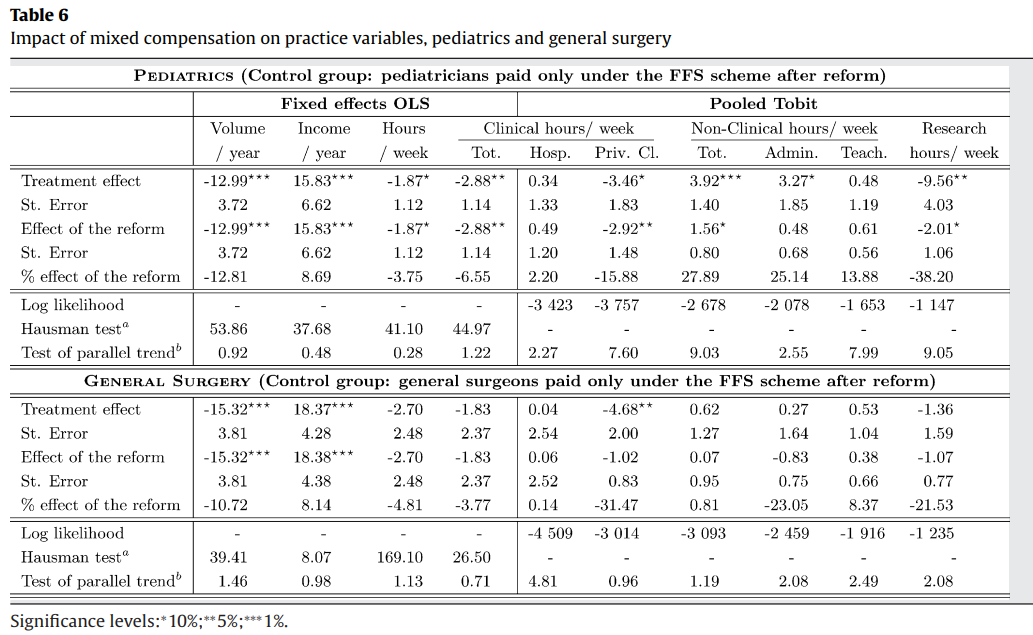
\includegraphics[width=0.9\textwidth]{pictures/multitask_doctors.png}
\end{frame}

\begin{frame}{The One Task Assumption}
    \begin{wideitemize}
        \item So far we have assumed that there is a single, productive task.
        \item This captures many jobs and environments well.
        \item The trade-off is between exerting effort and not exerting effort.
        \item But some jobs have more than one type of productive effort.
        \begin{wideitemize}
            \item Question: Can you give examples?
        \end{wideitemize}
        \item Some jobs have destructive tasks!
        \begin{wideitemize}
            \item Question: Can you give examples?
        \end{wideitemize}
    \end{wideitemize}
\end{frame}

\begin{frame}{The Multitasking Model: Dropping Uncertainty}
    \begin{wideitemize}
        \item We want to capture a new force (multiple tasks)
        \item To keep things simple, we drop noise/luck/uncertainty ($\epsilon$)
        \item We no longer need to think about certainty equivalents, variances, etc.
        \item We also will assume an outside option of 0 for the worker.
    \end{wideitemize}
\end{frame}

\begin{frame}{The Multitasking Model: Adding Multiple Tasks}
    \begin{wideitemize}
        \item The worker will have two tasks, numbered 1 and 2.
        \item The cost of exerting effort $e_1$ at task 1 and $e_2$ will be $c(e_1, e_2)$
        \item We will assume this function is increasing in each argument, but not much else.
        \item Output is given by $y=a e_1 + b e_2$, where $a,b$ can be positive or negative.
        \item We can only pay based on some measurement of effort: $m(e_1, e_2)$
    \end{wideitemize}
\end{frame}


\section{Crowding Out}

\begin{frame}{Model}
\begin{wideitemize}
    \item Output is $y=a e_1+b e_2, a>0, b>0$
    \item Cost of effort is:
       \[c(e_1, e_2) = \begin{cases}
            0 & \text{ if }  e_1+e_2 \leq 2 \bar e \\
            (e_1+e_2-2\bar e)^2/2 & \text{ if } e_1+e_2 \geq 2 \bar e 
        \end{cases}\]
    \item Only task 1 effort is measured: $m=e_1$
    \item Only what is measured is rewarded: $w(m)=\alpha + \beta m =\alpha + \beta e_1$
\end{wideitemize}
    
\end{frame}


\begin{frame}{First-Best Solution}
\centering
    \huge See the board!
\end{frame}

\begin{frame}{Equilibrium Solution (What Actually Happens)}
\centering
    \huge See the board!
\end{frame}

\begin{frame}{Equilibrium Solution (What Actually Happens)}
\begin{theorem}
    The firm uses high-powered incentives ($\beta^*=a$) and the worker focuses entirely on task 1 ($e_1^*=a + 2\bar e, e_2^*=0$) if:
\[a \geq 2\bar e\frac{ b - a }{a}\]
    Otherwise the firm uses a flat salary ($\beta^*=0$) and total effort is low and evenly split ($e_1^*=e_2^*=\bar e$)
\end{theorem}
\end{frame}


\begin{frame}{Deepwater Horizon}

\begin{wideitemize}
    \item Cost reductions were rewarded ($e_1$).
    \item But improving ``safety" or ``latent risk" was not.
    \item Part of this is not nefarious: cost reductions are easy to measure.
    \item Avoided disasters are impossible to measure!
    \item In some instances incentives are worse than no incentives!
\end{wideitemize}

\end{frame}
% \begin{frame}{The Multitasking Model Variants}
%     \begin{wideitemize}
%         \item "Crowding Out":
%         \[c(e_1, e_2) = \begin{cases}
%             0 & \text{ if }  e_1+e_2 \leq 2 \bar e \\
%             (e_1+e_2-2e)^2/2 & \text{ if } e_1+e_2 \geq 2 \bar e 
%         \end{cases}\]
%         \[m = e_1\]
%         \[a>0, b>0\]
%         \item "Destructive Effort"
%         \[c(e_1, e_2) = (e_1^2+e_2^2)/2 \]
%         \[m = e_1+e_2\]
%         \[a>0, b<0\]
%     \end{wideitemize}
% \end{frame}


% \begin{frame}{The Multitasking Model Variants}
%     \begin{wideitemize}
%         \item "Crowding Out":
%         \[c(e_1, e_2) = \begin{cases}
%             0 & \text{ if }  e_1+e_2 \leq 2 \bar e \\
%             (e_1+e_2-2e)^2/2 & \text{ if } e_1+e_2 \geq 2 \bar e 
%         \end{cases}\]
%         \[m = e_1\]
%         \[a>0, b>0\]
%         \item "Destructive Effort"
%         \[c(e_1, e_2) = (e_1^2+e_2^2)/2 \]
%         \[m = e_1+e_2\]
%         \[a>0, b<0\]
%     \end{wideitemize}
% \end{frame}

\begin{frame}{Counterterrorism at the FBI}
    \begin{wideitemize}
        \item The FBI was created to fight traditional crime, like murders.
        \item Traditional crime is easy to measure:
        \begin{wideitemize}
            \item How many suspects did you bring in?
            \item How much evidence did you collect?
            \item Was there a conviction?
        \end{wideitemize}
        
    \end{wideitemize}
\end{frame}


\begin{frame}{Counterterrorism at the FBI}
    \begin{wideitemize}
         \item During the 1990s, the FBI tried to also handle domestic terrorism.
        \item But how do you measure this?
        \item Terrorism is rare.
        \item Successful counterterrorism prevents things from happening.
    \end{wideitemize}
\end{frame}


\section{Teaching to the Test?}

\begin{frame}
\centering
    \huge Discussion: Lavy (2009)

\end{frame}



\begin{frame}{``Screening with Multitasking" (Dinerstein and Opper 2023)}
 \begin{wideitemize}
     \item Still a working paper. Main focus is on screening.
     \item However, the paper shows evidence of multitasking or teaching to the test.
     \item NYC increased weight on test scores for teacher tenure.
     \item Teacher valued-added for test scores rose, while teacher value-added for attendance and grades fell.
     \item However tenure became a more effective sorting mechanism: they got better teachers (main focus of paper).
 \end{wideitemize}
%https://www.nber.org/papers/w30310

\end{frame}


\begin{frame}[c]{``Screening with Multitasking" (Dinerstein and Opper 2023)}
\centering
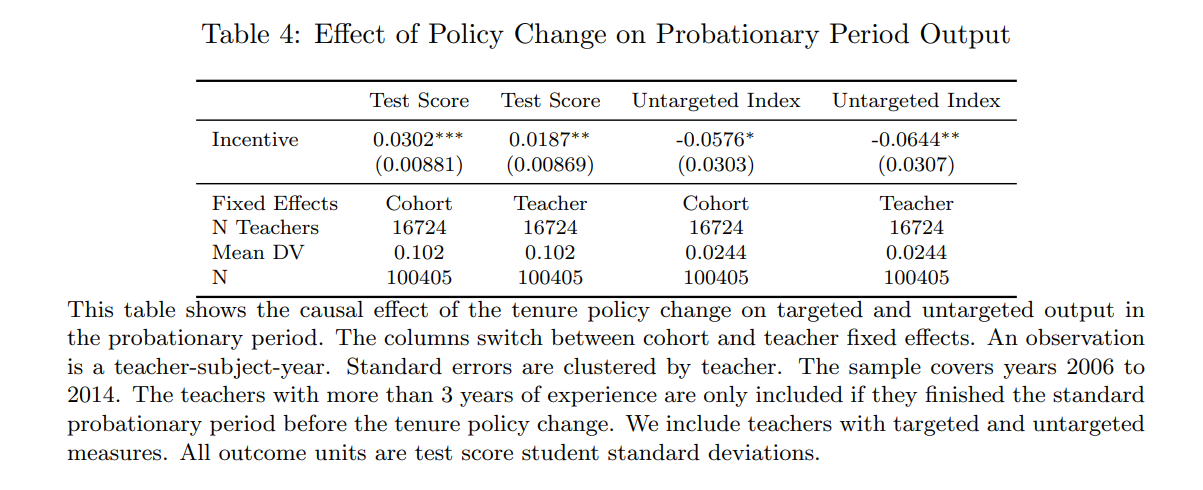
\includegraphics[width=0.9\textwidth]{pictures/teacher_multitasking.png}

``Untargeted" includes attendance, grades and graduation, while "targeted" are the test scores.
\end{frame}

       
\end{document}







